\documentclass[12pt]{article}
\usepackage[T1]{fontenc}
\usepackage{graphicx}
\usepackage{float}
\usepackage[polish]{babel}
\usepackage{amsmath}

\setlength{\textheight}{21cm}

\title{{\bf Zadanie nr 4 - Przekształcenia Fouriera, Walsha-Hadamarda, kosinusowe i falkowe, szybkie algorytmy}\linebreak
Cyfrowe Przetwarzanie Sygnałów}
\author{Jakub Wąchała, 216914 \and Radosław Grela, 216769}
\date{09.05.2020}

\begin{document}
\clearpage\maketitle
\thispagestyle{empty}
\newpage
\setcounter{page}{1}
\section{Cel zadania}
\label{cel}
Celem zadania jest oswojenie się z zagadnieniami dotyczącymi przekształceń Fouriera,Walsha-Hadamarda, kosinusowych i falkowych oraz szybkich algorytmów. Zadanie polega na implementacji dodatkowych funkcjonalności do naszej aplikacji: rysowanie sygnałów o wartościach zespolonych oraz transformacje dyskretne i falkowe \cite{bib1}

\section{Wstep teoretyczny}
Program ten jest wzbogaconą wersją programu z zadania 1., 2., 3. Umożliwia wykonanie operacji przekształceń,  rysowanie sygnałów o wartościach zespolonych oraz transformacje dyskretne i falkowe.

\subsection {Zaimplementowane warianty:}
\begin {enumerate}
\item Tryby prezentacji wykresów:
\begin {itemize}
\item (W1) – górny wykres prezentuje część rzeczywistą amplitudy w funkcji częstotliwości, a wykres dolny część urojoną;
\item (W2) – górny wykres prezentuje moduł liczby zespolonej, a dolny argument liczby w funkcji częstotliwości.
\end {itemize}
\item Transformacje sygnałów
\begin {itemize}
\item Dyskretna transformacja Fouriera – algorytm z definicji oraz szybka transformacja Fouriera;
\item Tansformacja falkowa, wariant DB4
\end {itemize}
\end{enumerate}

\section{Eksperymenty i wyniki}
Eksperymenty zostały przez nas podzielone na: prezentacje wykresów W1, W2, transformacje sygnałów.  
\\
Skorzystamy z funkcji sinusoidalnej z parametrami:
\begin{itemize}
\item amplituda: 1
\item okres: 1
\item czas początkowy: 0
\item czas trwania: 10
\end{itemize}
A także z sygnału S1.
\subsection{Sygnał S1}

\begin{figure}[H]
\centering
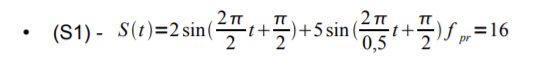
\includegraphics[scale=0.6]{sygnalS1.png}
\caption{Funkcja opisująca sygnał S1}
\end{figure}

\begin{figure}[H]
\centering
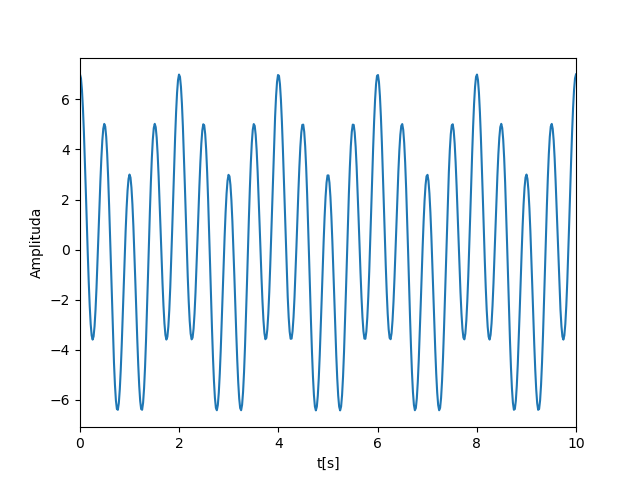
\includegraphics[scale=0.6]{sygnalS1rysunek.png}
\caption{Sygnał S1 wykorzystany do przedstawienia transformacji i rysunków}
\end{figure}


\subsection{Dyskretna transformacja Fouriera - sygnał sinusoidalny}
\begin{figure}[H]
\centering
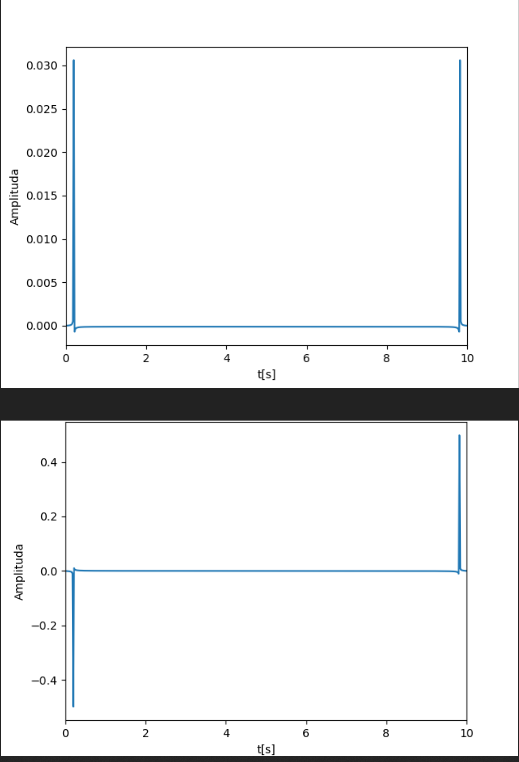
\includegraphics[scale=0.6]{sinusDyskrW1.png}
\caption{Dyskretna transformacja Fouriera W1 - sygnał sinusoidalny}
\end{figure}

\begin{figure}[H]
\centering
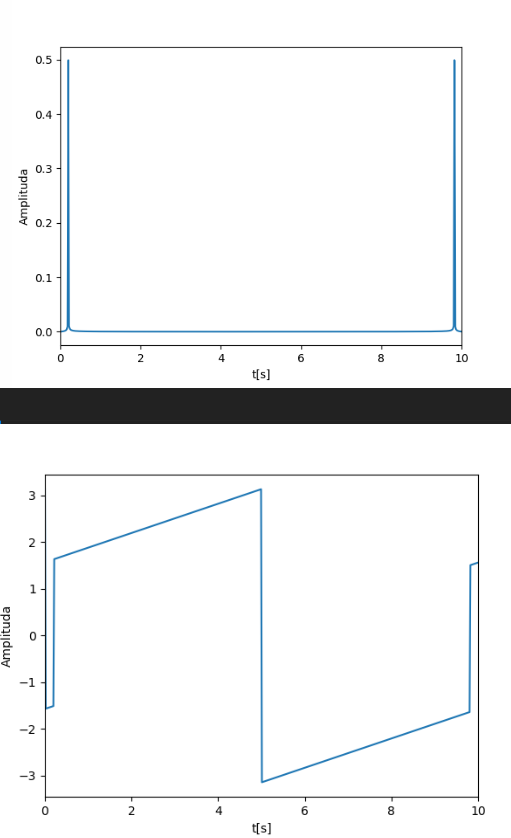
\includegraphics[scale=0.6]{sinusDyskrW2.png}
\caption{Dyskretna transformacja Fouriera W2 - sygnał sinusoidalny}
\end{figure} 

\subsection{Dyskretna transformacja Fouriera - sygnał S1}
\begin{figure}[H]
\centering
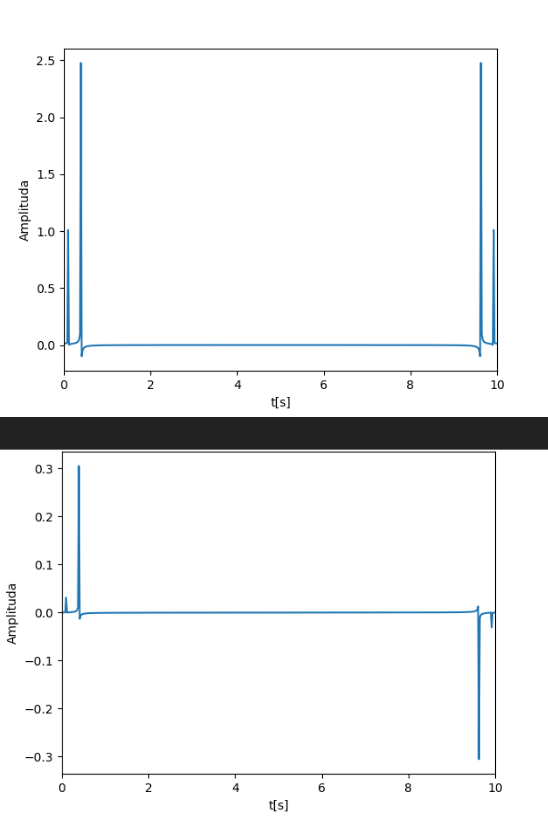
\includegraphics[scale=0.6]{s1DyskrW1.png}
\caption{Dyskretna transformacja Fouriera W1 - sygnał S1}
\end{figure}

\begin{figure}[H]
\centering
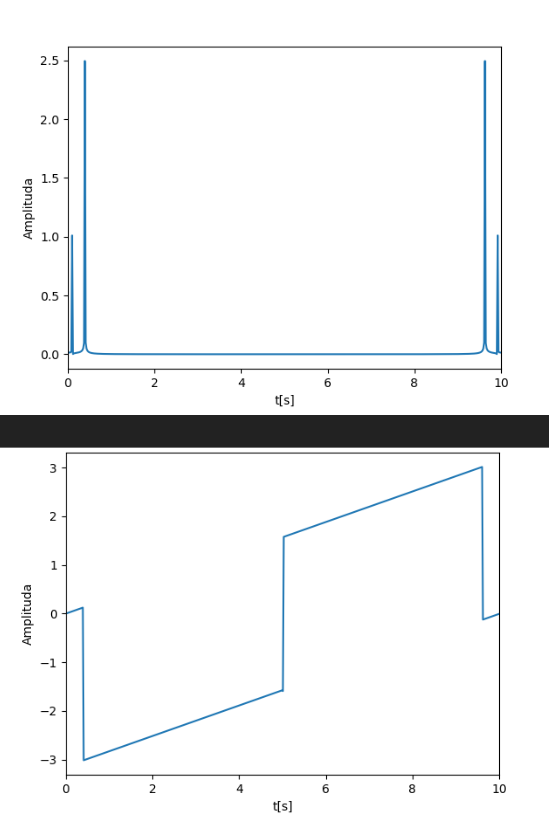
\includegraphics[scale=0.6]{s1DyskrW2.png}
\caption{Dyskretna transformacja Fouriera W2 - sygnał S1}
\end{figure} 

\subsection{Szybka transformacja Fouriera - sygnał sinusoidalny}

\begin{figure}[H]
\centering
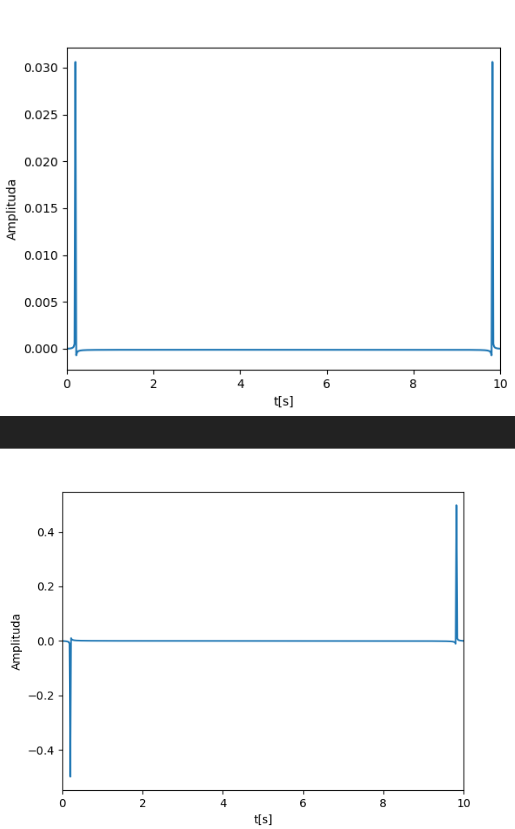
\includegraphics[scale=0.6]{sinusFastW1.png}
\caption{Szybka transformacja Fouriera W1 - sygnał sinusoidalny}
\end{figure}

\begin{figure}[H]
\centering
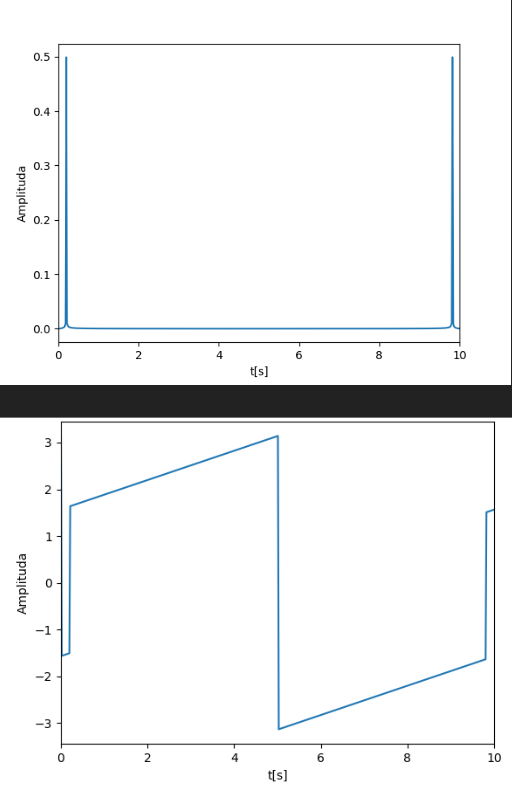
\includegraphics[scale=0.6]{sinusFastW2.png}
\caption{Szybka transformacja Fouriera W2 - sygnał sinusoidalny}
\end{figure}

\subsection{Szybka transformacja Fouriera - sygnał s1}

\begin{figure}[H]
\centering
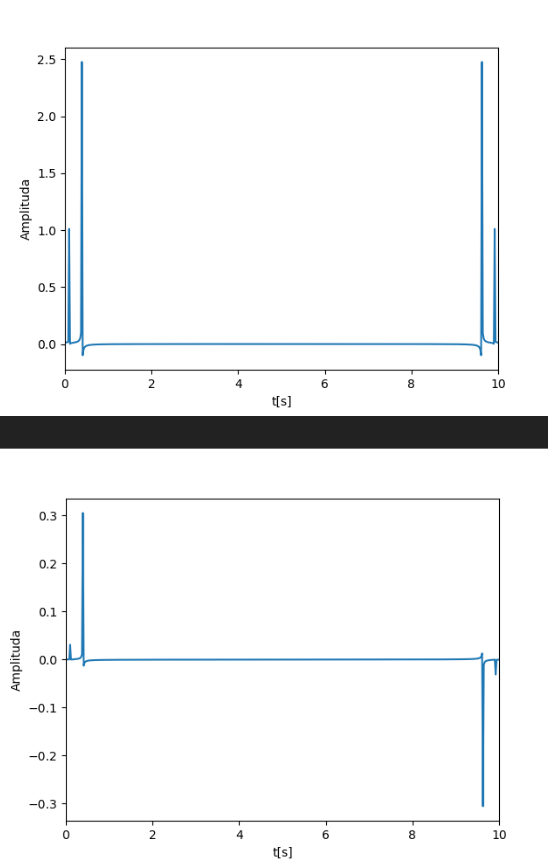
\includegraphics[scale=0.6]{s1FastW1.png}
\caption{Szybka transformacja Fouriera W1 - sygnał s1}
\end{figure}

\begin{figure}[H]
\centering
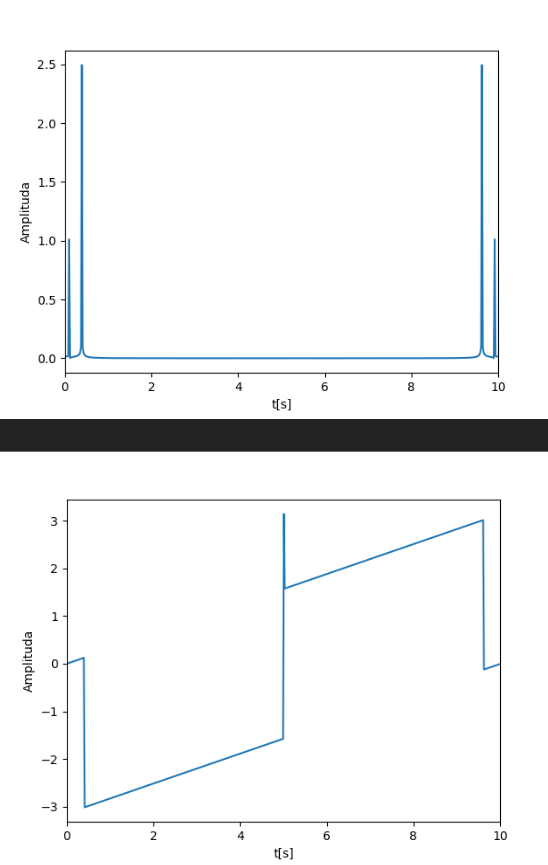
\includegraphics[scale=0.6]{s1FastW2.png}
\caption{Szybka transformacja Fouriera W2 - sygnał s1}
\end{figure}


\subsection{Zestawienie czasów dyskretnej i szybkiej transformaty Fouriera}


\begin{itemize}
\item Sygnał sinusoidalny (5 uruchomień programu)


\begin{tabular}{|r|l|}
  \hline 
  Dyskr. transf. Fouriera & Szybka transf. Fouriera \\
  \hline
  0.391950 s & 0.008976 s \\
  \hline
  0.327151 s &  0.009972 s \\
  \hline
  0.350166 s & 0.007978 s \\
  \hline
  0.338912 s &0.008977 s \\
  \hline
  0.332111 s & 0.010003 s \\
  \hline
\end{tabular} 

\item Sygnał s1 (5 uruchomień programu)

\begin{tabular}{|r|l|}
  \hline 
  Dyskr. transf. Fouriera & Szybka transf. Fouriera \\
  \hline
  0.350071 s & 0.013932 s \\
  \hline
  0.323501 s & 0.009993 s \\
  \hline
  0.347075 s &0.009973 s \\
  \hline
  0.325157 s & 0.011967 s \\
  \hline
   0.373002 s & 0.008976 s \\
  \hline
\end{tabular} 

\end{itemize}

\subsection{Transformacja falkowa wariant - DB4}
\begin{figure}[H]
\centering
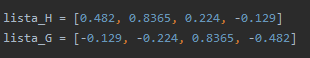
\includegraphics[scale=0.99]{listaHG.png}
\caption{Elementy filtru H i G (DB4)}
\end{figure}


\begin{figure}[H]
\centering
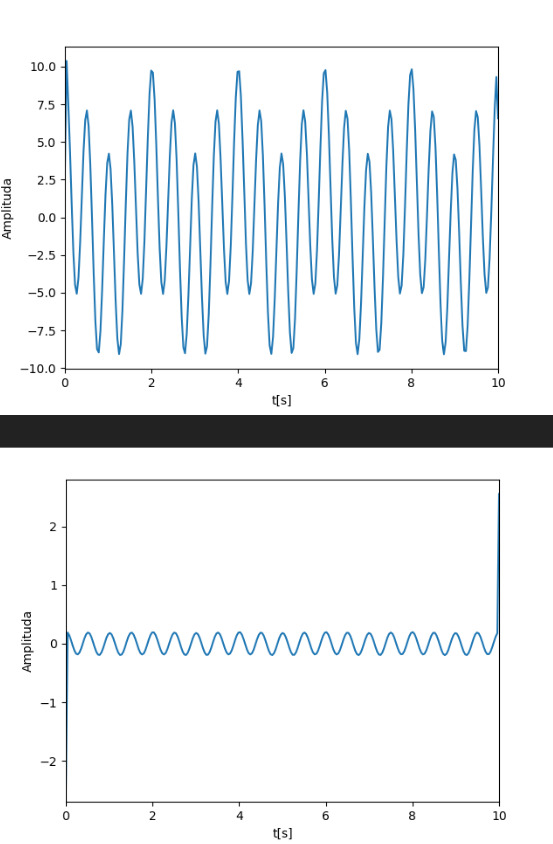
\includegraphics[scale=0.6]{s1FalkaW1.png}
\caption{Transformacja falkowa  W1}
\end{figure}

\begin{figure}[H]
\centering
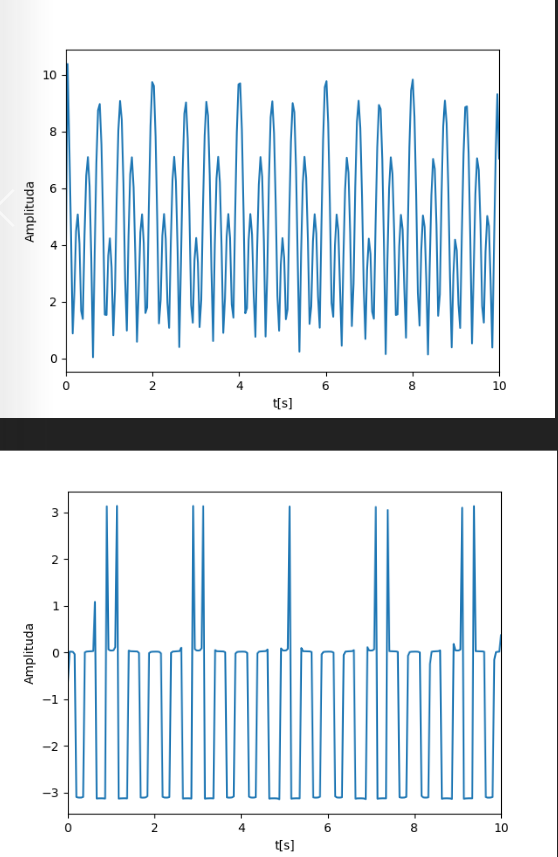
\includegraphics[scale=0.6]{s1FalkaW2.png}
\caption{Transformacja falkowa W2}
\end{figure}

\begin{figure}[H]
\centering
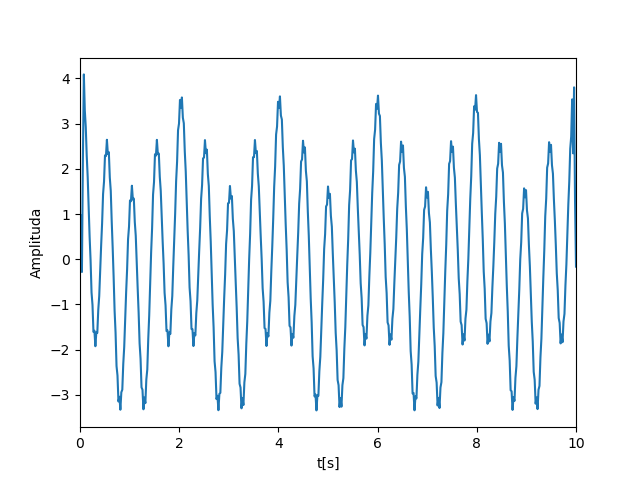
\includegraphics[scale=0.6]{s1FalkaOdwrocona.png}
\caption{Transformacja falkowa odwrotna}
\end{figure}

\section{Wnioski}
\begin {itemize}
\item Prezentowane wyniki są dowodem na poprawne wykonanie zadania tj. poprawność wykonania operacji transformacji, rysowania wykresów sygnałów zespolonych.
\item Szybka transformata Fouriera w znaczącym stopniu zmniejsza czas trwania algorytmu w porównaniu do dyskretnej tranformaty Fouriera
\item Wykorzystanie cech szybkiej transformaty Fouriera pozwala budować bardzo wydajne algorytmy
\end {itemize}


\begin{thebibliography}{0}
\bibitem{bib1} Instrukcja do zadania 4 - Przeksztaªcenie Fouriera, Walsha-Hadamarda, kosinusowe i falkowe, szybkie algorytmy https://ftims.edu.p.lodz.pl/pluginfile.php/14303/mod\_resource/content/0/zadanie4.pdf [dostęp 09.06.2020]

\end{thebibliography}

\end{document}